\documentclass[11pt]{beamer}
%\documentclass[handout,dvips,11pt,grey]{beamer}

\usepackage{multicol}
\usepackage{verbatim}
\usepackage{graphicx}


\begin{document}

\title{PPAML Summer School}

\subtitle{Geolocation Using Wifi Signal in Figaro}

\author{Sebastian Imlay, Daniel Salvadori, Philip M. Robinson}

\institute{PPAML}

\date{\today}

\begin{frame}
  \titlepage
\end{frame}


\begin{frame}{Domain Problem}

\end{frame}

\begin{frame}{Model Discussion and History}
\begin{center}
\begin{multicols}{3}
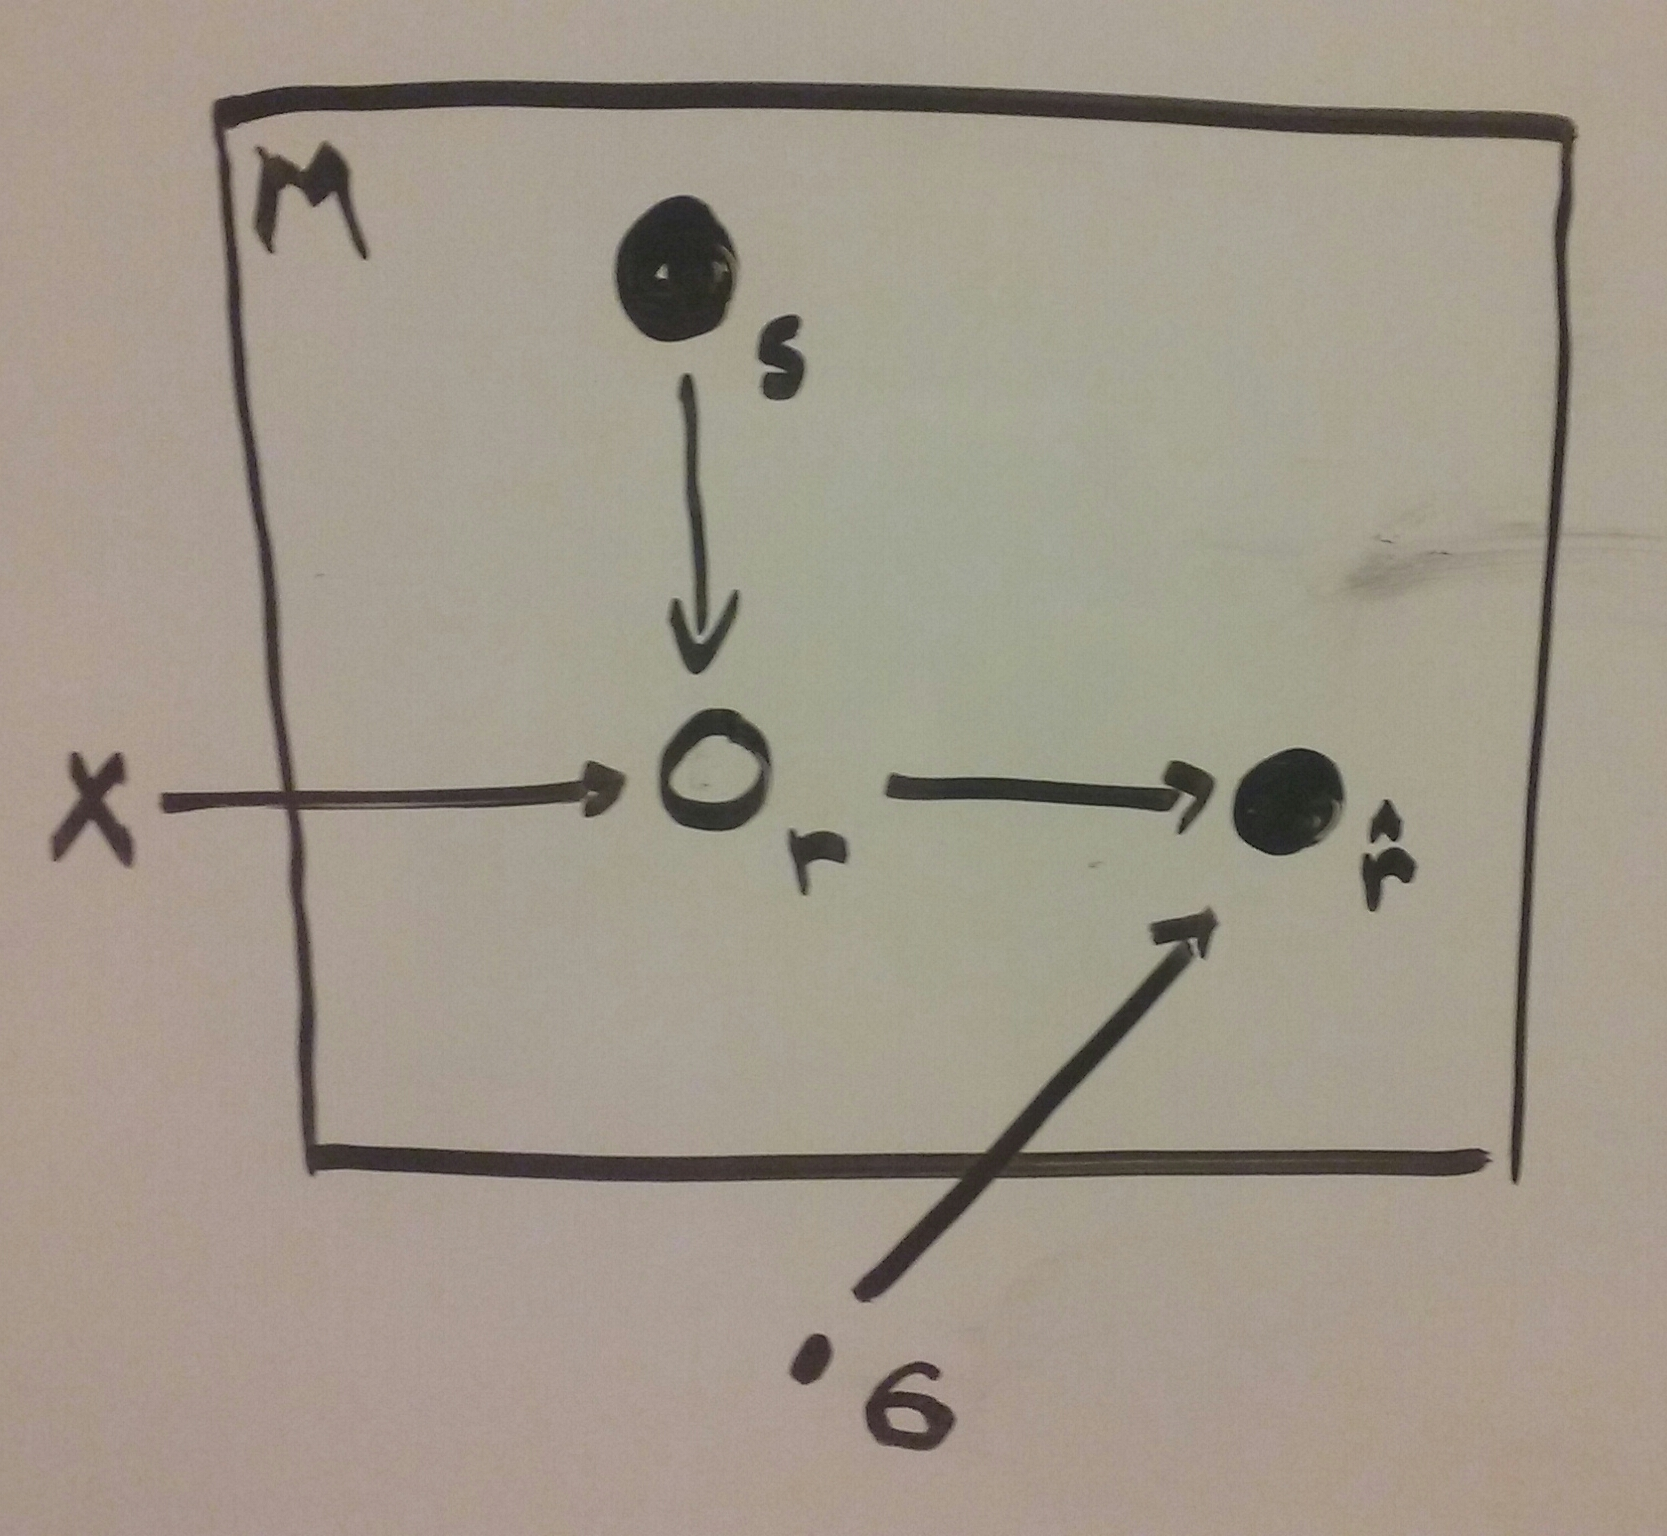
\includegraphics[height=1in]{pictures/1plate.jpg}

%abcd
\columnbreak

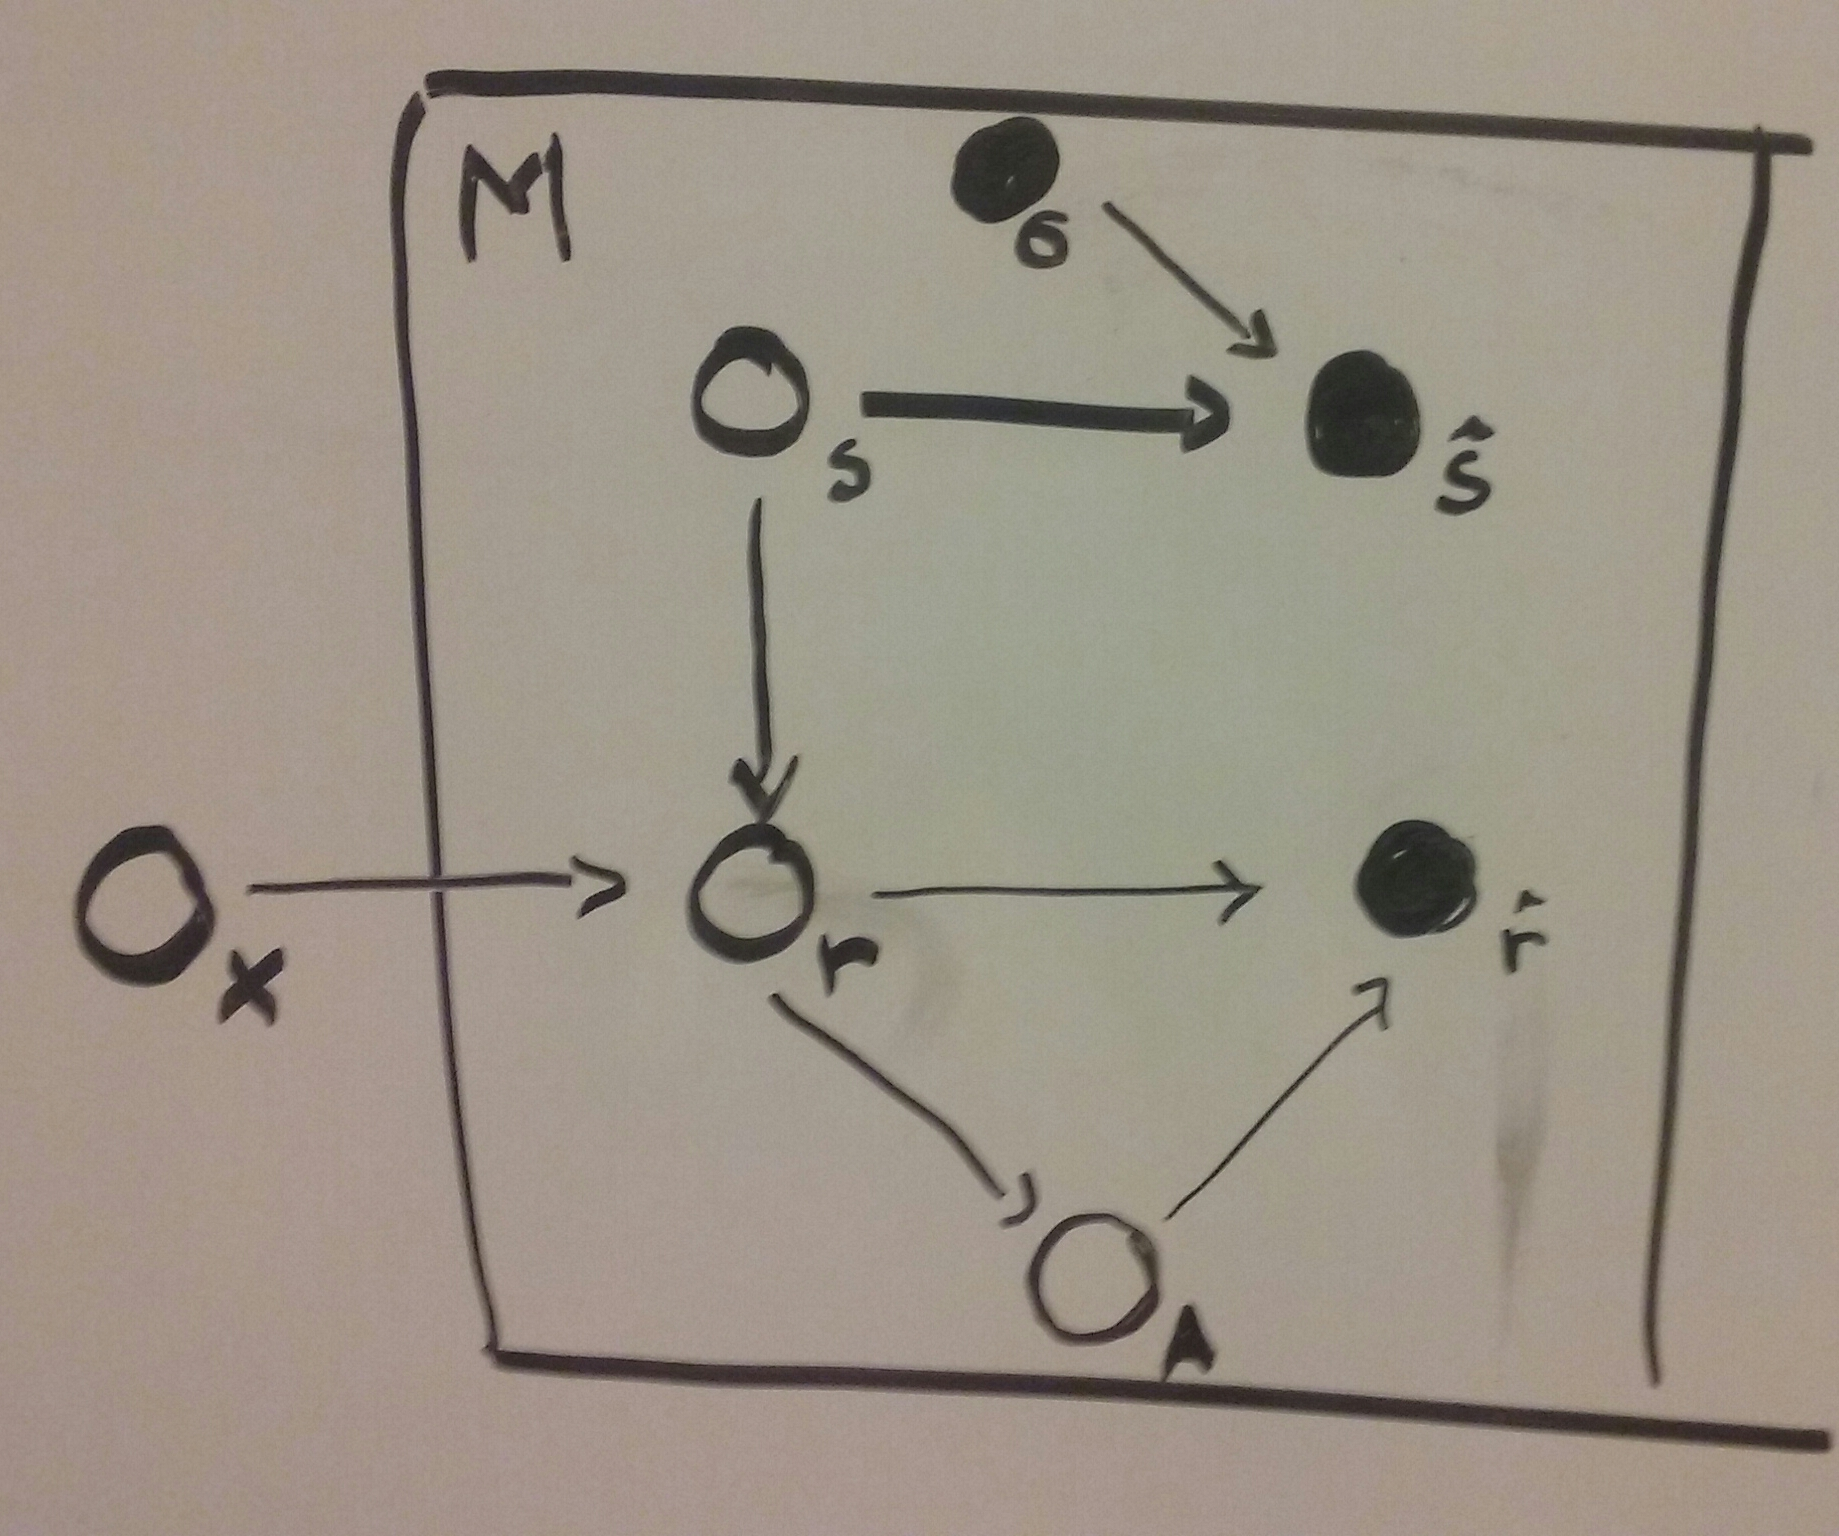
\includegraphics[height=1in]{pictures/2plate.jpg}

%abcd
\columnbreak

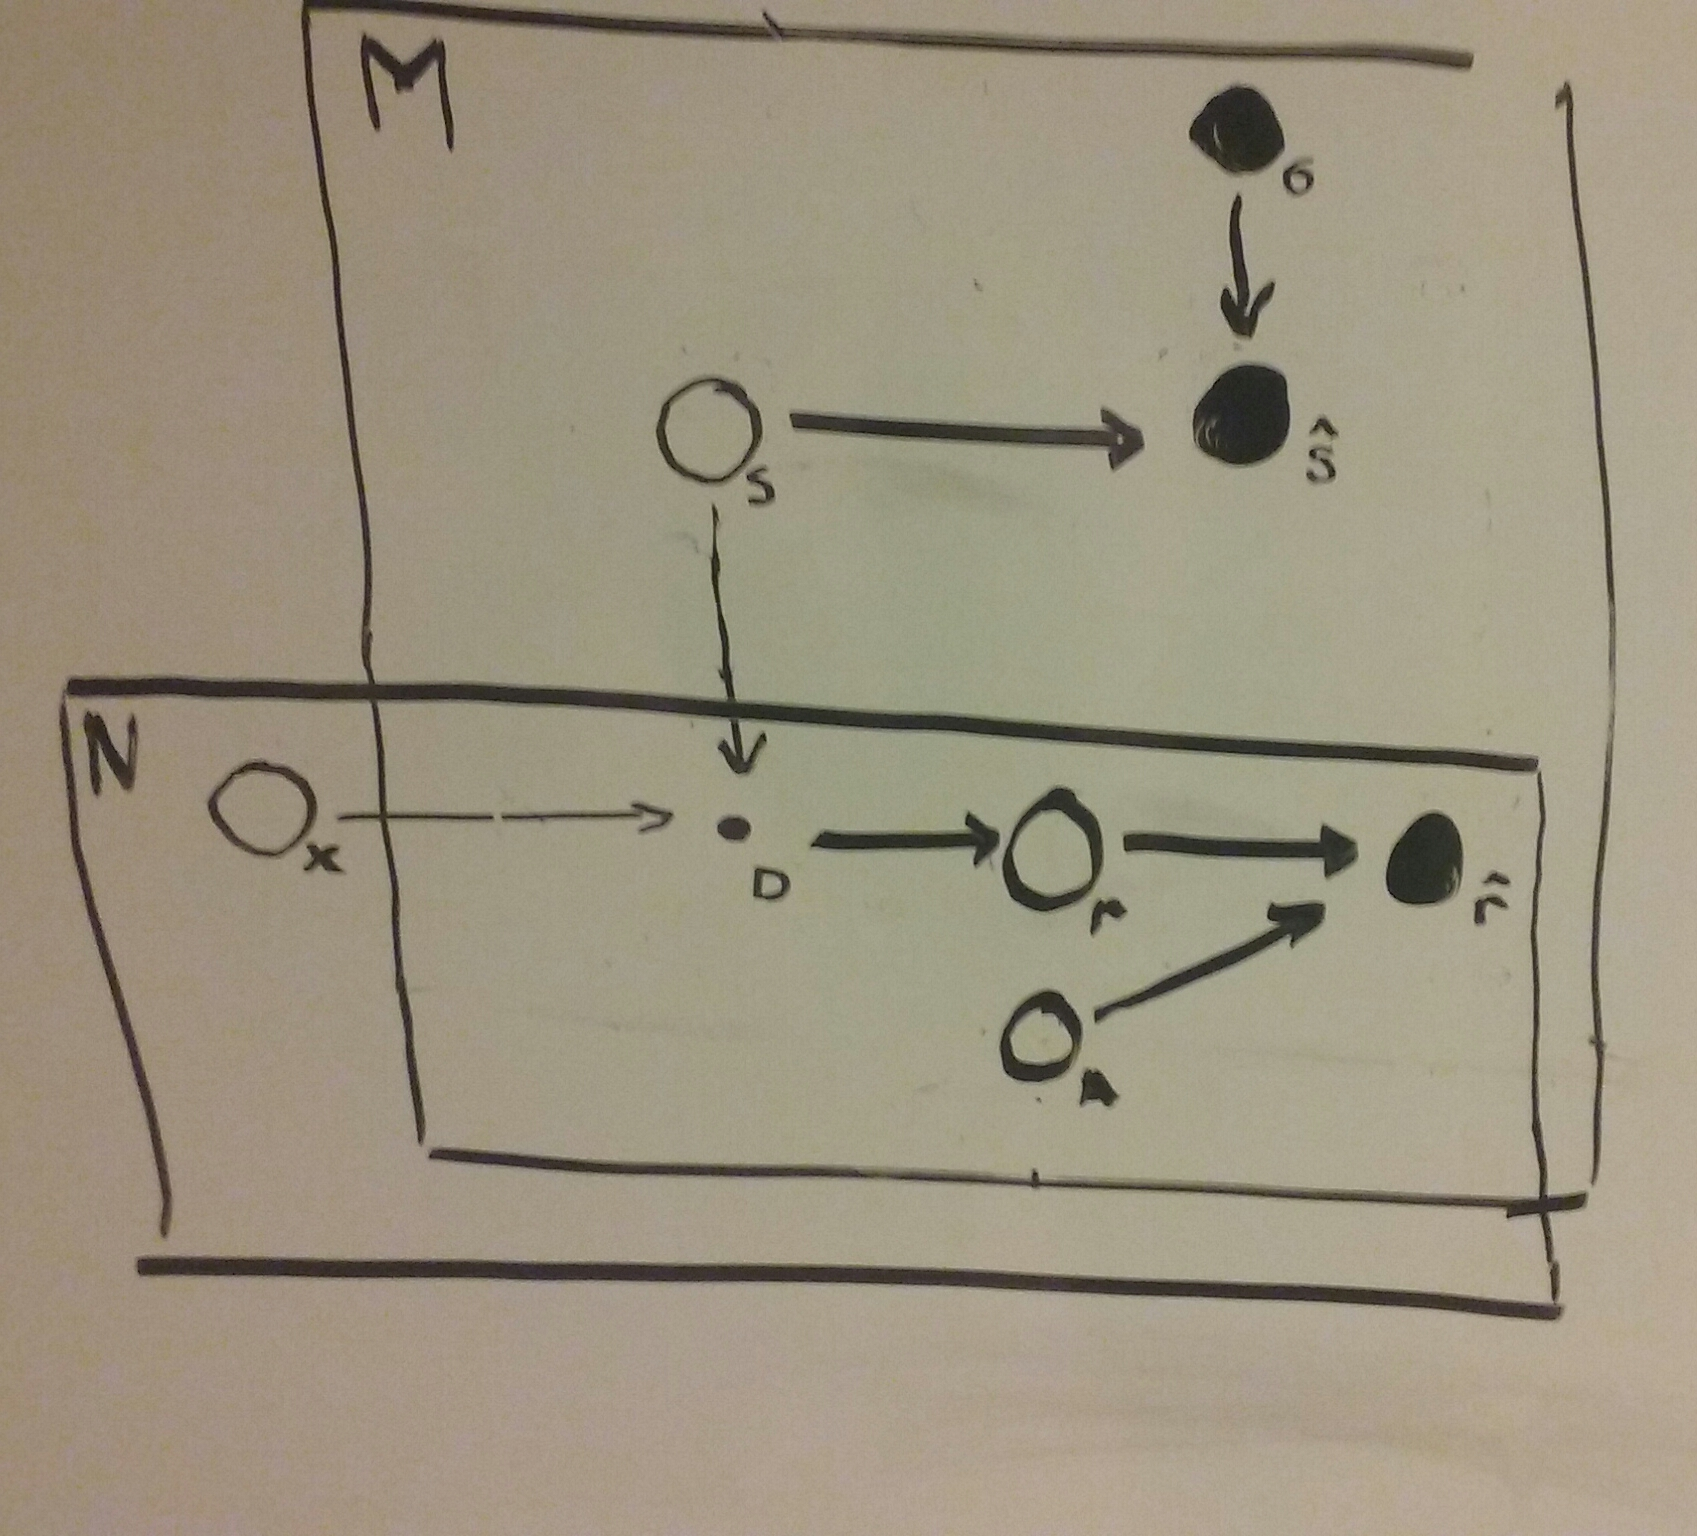
\includegraphics[height=1in]{pictures/3plate.jpg}

%abcd
\columnbreak
\end{multicols}
\end{center}
\begin{itemize}
\item[N] Transmitters
\item[M] Recievers
\item[S] Reciever Position
\item[X] Reciever Position
\item[r] Power
\item[A] Attinuation
\item[D] Distance
\end{itemize}

\end{frame}

\begin{frame}{Implementation - Supporting Technology}

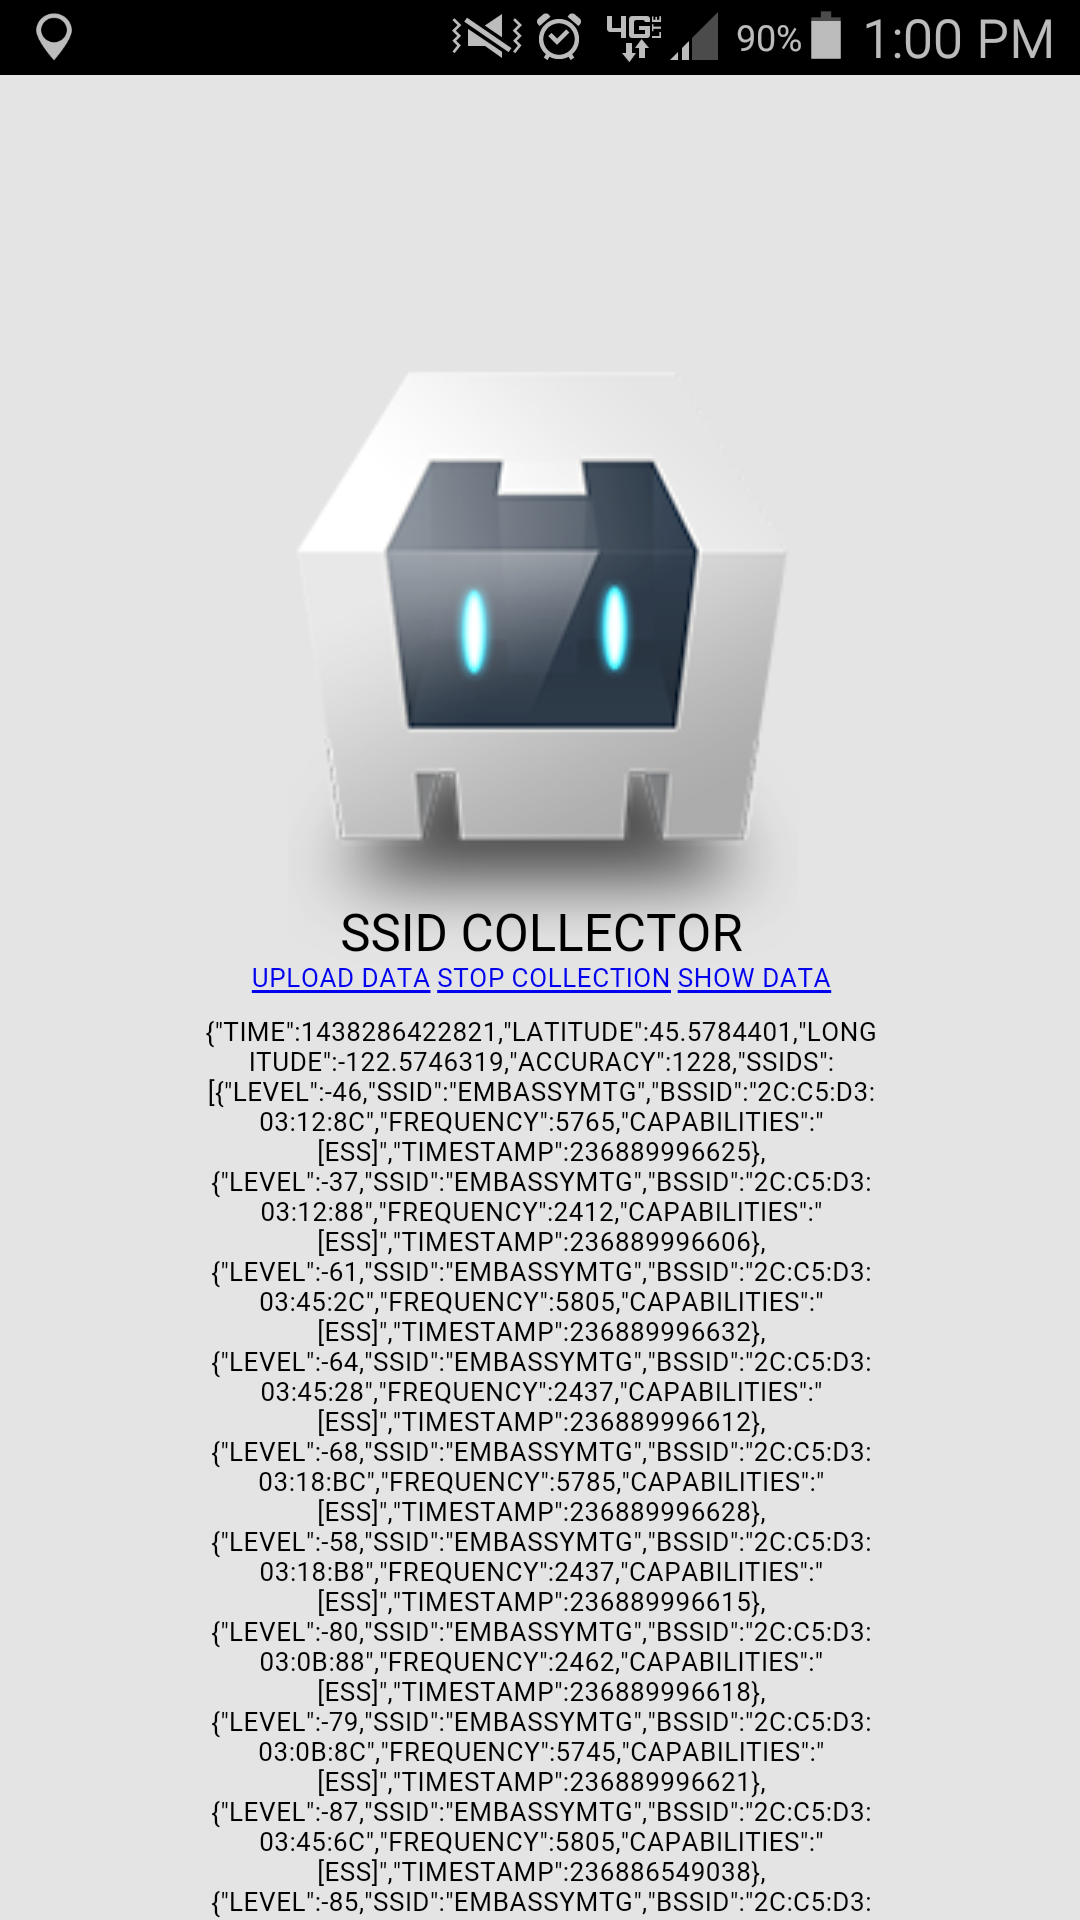
\includegraphics[height=0.7\textheight]{pictures/phoneapp.png}
\end{frame}

\begin{frame}{Implementation - Figaro}

\end{frame}

\begin{frame}{Insignts}

\end{frame}

\begin{frame}{Collateral}

\end{frame}

\end{document}
